\section{Diagrammi delle attività}
\label{diagrammiAtt}
Vengono di seguito illustrati i diagrammi di attività che descrivono l'interazione dell'utente, con l'applicativo \project{}. Il diagramma d'uso principale (fig. \ref{generale}) è stato suddiviso in sotto-diagrammi per ovvi motivi di spazio. I riquadri con sfondo bianco quindi, sono da considerarsi singole azioni, mentre quelli con sfondo azzurro sono attività ad alto livello.

\subsection{Attività principali}
\label{principle}
Una volta avviato il programma, l'utente può:
\begin{itemize}
\item\textbf{Avviare un'analisi};
\item\textbf{Creare:} nuovi \subject{}, nuovi gruppi di \subject{}, nuovi \protocol{} e nuovi \dataset{};
\item\textbf{Visualizzare:} i \subject{}, i gruppi di \subject{}, i \protocol{} e i \dataset{} presenti nel sistema, oltre ai risultati della analisi finora effettuate;
\item\textbf{Modificare:} i gruppi di \subject{} (aggiungendo o togliendo uno o più \subject{});
\item\textbf{Eliminare:} \protocol{} e \dataset{};
\item\textbf{Esportare:} i risultati delle analisi effettuate;
\item\textbf{Aprire:} la guida contestuale.
\end{itemize}
Le funzionalità sopra descritte, potranno essere sfruttate dall'utente in mutua esclusione. Una volta terminata l'azione che l'utente ha deciso di intraprendere, sarà per lui possibile sceglierne un'altra tra quelle proposte oppure chiudere l'applicativo.
\\
\\
Si evidenzia inoltre che, per mantenere una rappresentazione chiara, pulita e fluida delle attività, si è omesso il fatto che l'utente in ogni momento potrà chiudere il programma, accedere ad una voce del menù o ancora, annullare i passi fatti fino a quel momento ritornando alla pagina iniziale.
\pagebreak
\begin{landscape}
\begin{figure}[!h]
\centering
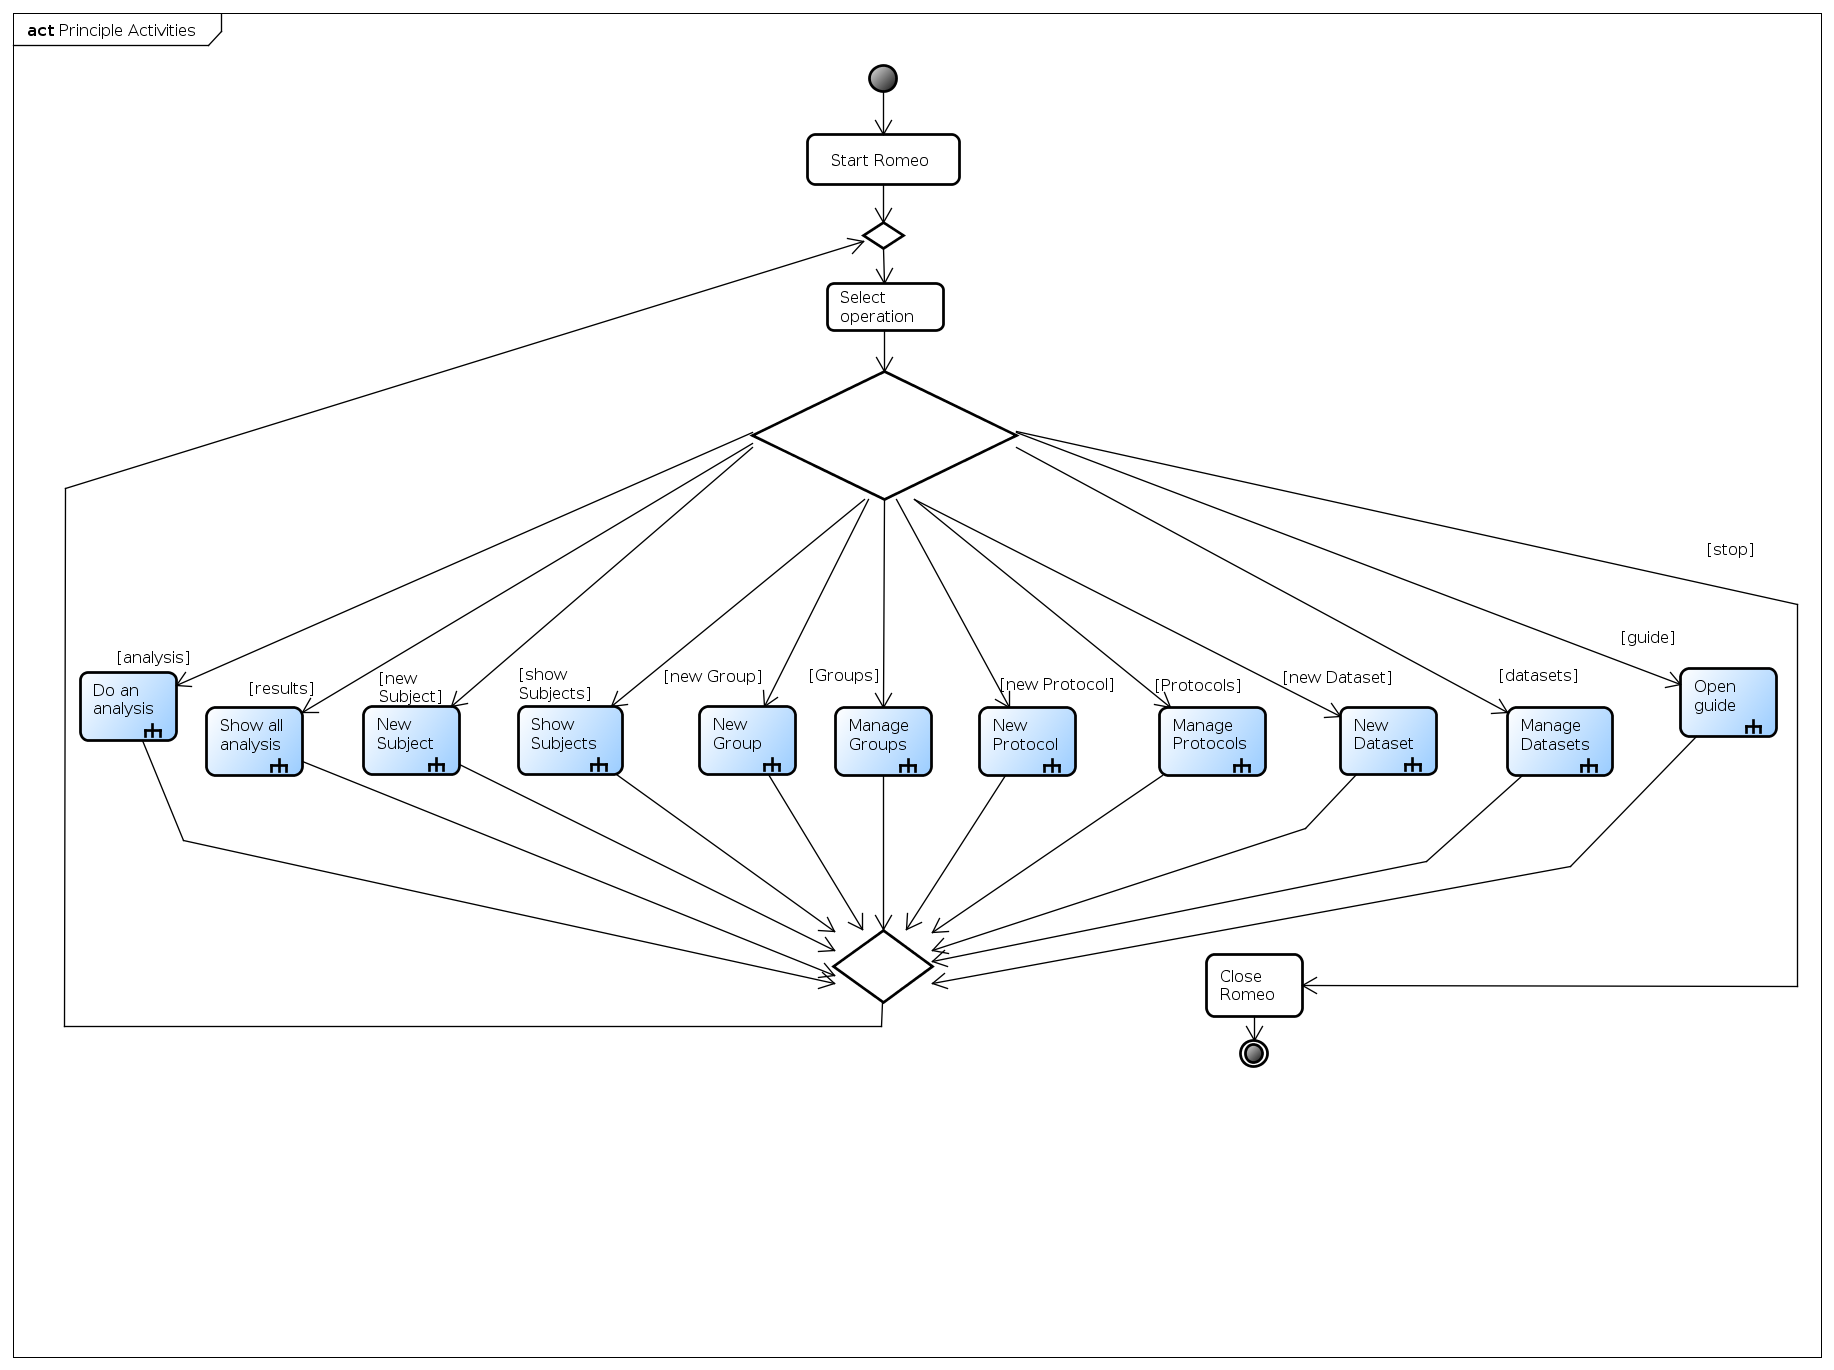
\includegraphics[width=0.9\linewidth]{./Content/Immagini/Principle_Activities}
\caption{Diagramma Attività - Attività principali dell'applicativo \project{}}
\label{generale}
\end{figure}
\end{landscape}
\pagebreak

% creare un nuovo subject
\subsection{New Subject}
\label{newSub}
\begin{figure}[!h]
\centering
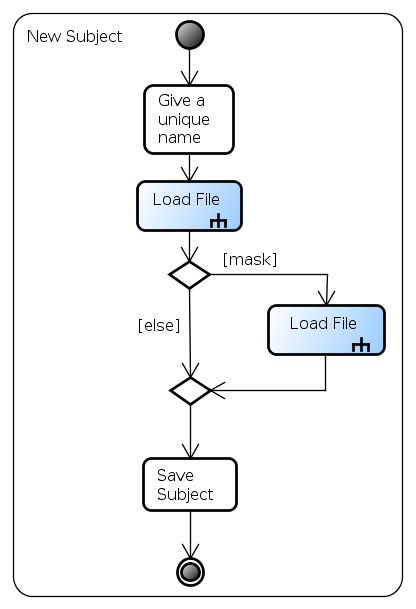
\includegraphics[width=0.6\linewidth]{./Content/Immagini/New_Subject}
\caption{Diagramma Attività - Creazione nuovo Subject}
\label{newS}
\end{figure}
\paragraph{Descrizione\\}
L'attività di creazione di un nuovo Subject\glossario{} (fig. \ref{newS}), prevede innanzitutto l'assegnazione di un nome univoco al \subject{} in creazione. Successivamente è necessario caricare il file, che può essere un'immagine o un video, ed eventualmente caricare una sua maschera. Infine, si procede con il salvataggio del \subject{}.
\pagebreak

%caricamento di un file in romeo
\subsubsection{Load File}
\label{LoadF}
\begin{figure}[!h]
\centering
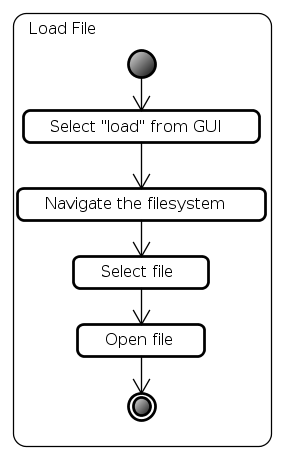
\includegraphics[width=0.4\linewidth]{./Content/Immagini/Load_File}
\caption{Diagramma Attività - Caricamento di un file}
\label{Load}
\end{figure}
\paragraph{Descrizione\\}
L'attività di caricamento di un file (fig. \ref{Load}), prevede la navigazione all'interno del filesystem e la selezione del file che si desidera caricare. Infine, dopo la conferma dell'utente, si procede con l'apertura dello stesso.
\pagebreak

%creazione di un nuovo gruppo
\subsection{New Group}
\label{newGr}
\begin{figure}[!h]
\centering
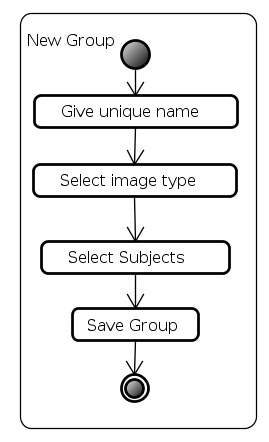
\includegraphics[width=0.4\linewidth]{./Content/Immagini/New_Group}
\caption{Diagramma Attività - Creazione nuovo gruppo di Subject}
\label{newGroup}
\end{figure}
\paragraph{Descrizione\\}
L'attività di creazione di un nuovo gruppo di Subject\glossario{} (fig. \ref{newGroup}), prevede in primo luogo l'assegnazione di un nome univoco al gruppo e la scelta del tipo d'immagine (2D, 2D-t, 3D o 3D-t) che si vuole utilizzare. Successivamente è necessario selezionare i Subject\glossario{} da inserire nel gruppo, scegliendo tra quelli che hanno un'immagine associata del tipo precedentemente scelto. Infine si procede con il salvataggio del gruppo.
\pagebreak

%creazione di un nuovo protocollo
\subsection{New Protocol}
\label{newPr}
\begin{figure}[!h]
\centering
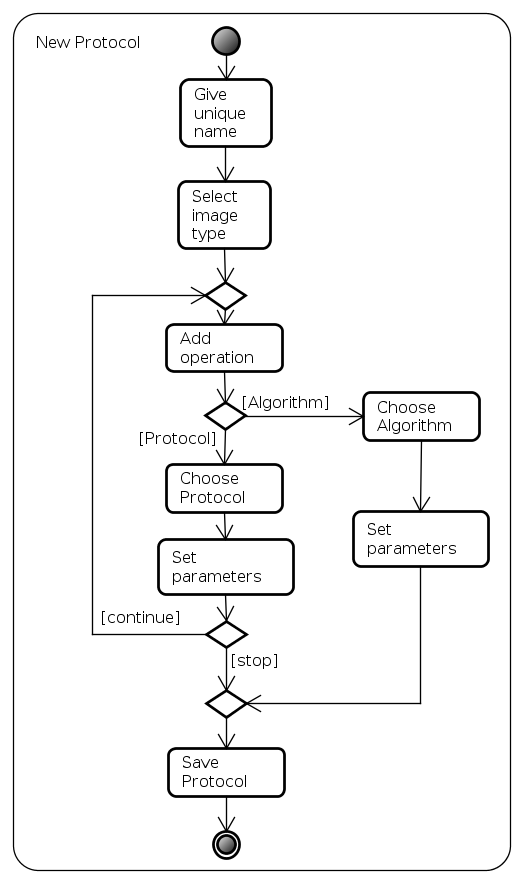
\includegraphics[width=0.6\linewidth]{./Content/Immagini/New_Protocol}
\caption{Diagramma Attività - Creazione di un nuovo Protocol}
\label{newProtocol}
\end{figure}
\paragraph{Descrizione\\}
L'attività di creazione di un nuovo Protocol\glossario{} (fig. \ref{newProtocol}), prevede in primo luogo l'assegnazione di un nome univoco al Protocol\glossario{} e la scelta del tipo di immagine a cui dovrà essere applicato. \`E possibile poi selezionare le feature extractors\glossario{} che si vogliono utilizzare, dando dei valori ai parametri richiesti, e/o selezionare l'algoritmo di clustering\glossario{} dando anche per esso, dei valori ai parametri richiesti. Qualora non vengano assegnati dei valori, verranno presi quelli di default previsti dal sistema. Una volta terminata la selezione, il Protocol\glossario{} è pronto per essere salvato.
\pagebreak

%creazione di un nuovo dataset
\subsection{New Dataset}
\label{newDataset}
\begin{figure}[!h]
\centering
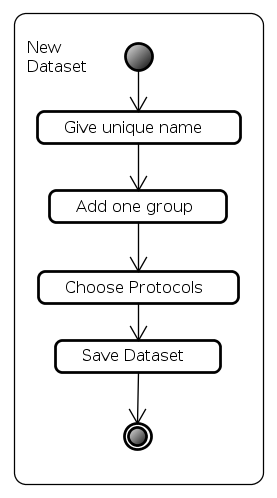
\includegraphics[width=0.4\linewidth]{./Content/Immagini/New_Dataset}
\caption{Diagramma Attività - Creazione di un nuovo Dataset}
\label{newData}
\end{figure}
\paragraph{Descrizione\\}
L'attività di creazione di un nuovo Dataset\glossario{} (fig. \ref{newData}), prevede in primo luogo l'assegnazione di un nome univoco al Dataset\glossario{} in creazione e l'inserimento, in quest'ultimo, di un unico gruppo di \subject{}. Successivamente, è necessario scegliere uno o più protocol\glossario{} da applicare al gruppo di \subject{}. I \protocol{} che potranno essere associati, saranno solo quelli compatibili in base al tipo di immagine del gruppo. Creata quest'associazione, il \dataset{} è pronto per essere salvato.
\pagebreak

%visualizzazione subjects
\subsection{Show Subjects}
\label{showSub}
\begin{figure}[!h]
\centering
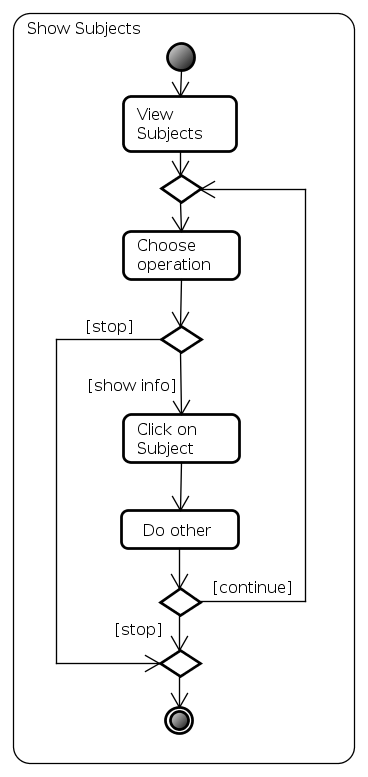
\includegraphics[width=0.5\linewidth]{./Content/Immagini/Show_Subjects}
\caption{Diagramma Attività - Visualizzazione dei Subject}
\label{showS}
\end{figure}
\paragraph{Descrizione\\}
L'utente avrà a disposizione l'elenco di tutti i Subject\glossario{} creati fino a quel momento. Selezionandone uno, potrà avere un'anteprima dell'immagine associata, assieme ad alcuni valori di interesse, come per esempio il tipo di immagine e la data di creazione.
\pagebreak

%gestione gruppi di subject
\subsection{Manage Groups}
\label{ManageGr}
\begin{figure}[!h]
\centering
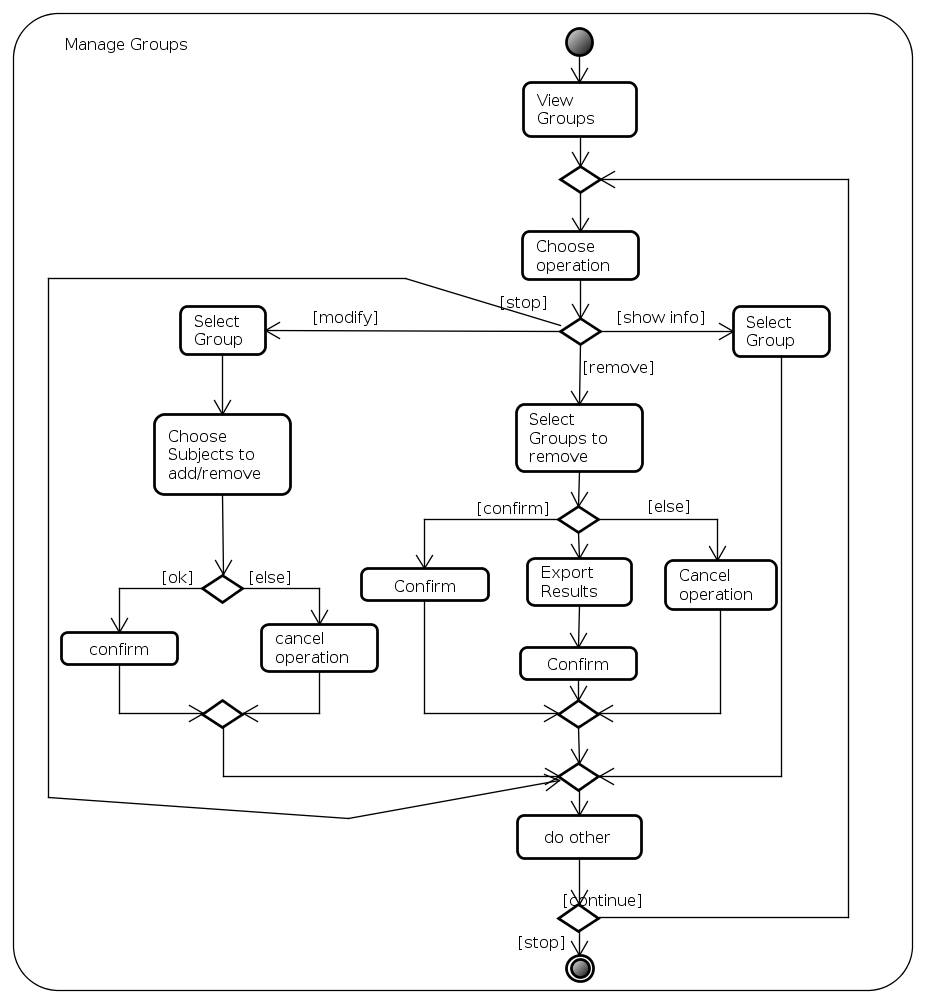
\includegraphics[width=\linewidth]{./Content/Immagini/Manage_Groups}
\caption{Diagramma Attività - Gestione dei gruppi di Subject}
\label{ManageG}
\end{figure}
\paragraph{Descrizione\\}
L'attività di gestione dei gruppi di Subject\glossario{} (fig. \ref{ManageG}), dà innanzitutto la possibilità all'utente di visualizzare i gruppi salvati in quel momento nel sistema. Per ogni entità, l'utente può effettuare alcune operazioni citate di seguito.\\
\`E possibile rimuovere uno o più gruppi, visualizzarne le informazioni (Subject\glossario{} appartenenti, tipo di immagine, ecc\dots) e modificarlo. La modifica consiste nel selezionare il gruppo e scegliere quali \subject{} eliminare o inserire.\\
Per ogni singola operazione, è necessaria la conferma da parte dell'utente, che può inoltre annullarla in qualsiasi momento.
\pagebreak

%gestione dei protocolli
\subsection{Manage Protocols}
\label{ManageProt}
\begin{figure}[!h]
\centering
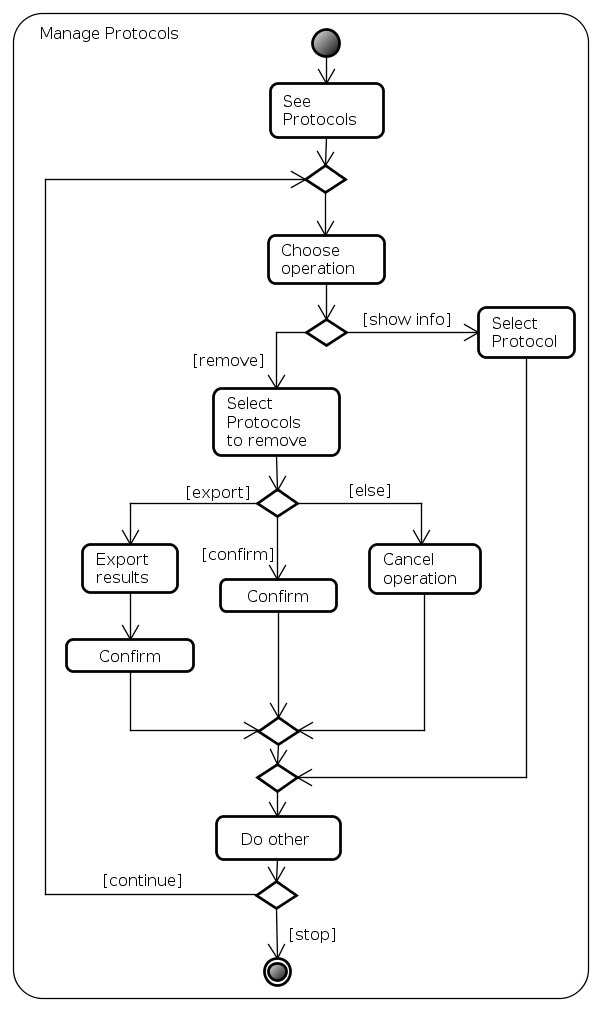
\includegraphics[width=0.8\linewidth]{./Content/Immagini/Manage_Protocols}
\caption{Diagramma Attività - Gestione dei Protocol}
\label{ManagePr}
\end{figure}
\paragraph{Descrizione\\}
L'attività di gestione dei Protocol\glossario{} (fig. \ref{ManagePr}), dà la possibilità all'utente di visualizzare i Protocol\glossario{} presenti in quel momento nel sistema. Per ogni \protocol{}, l'utente può decidere se visualizzarne le informazioni d'interesse o se rimuoverlo. La cancellazione di un \protocol{} necessita della conferma dell'utente.
\pagebreak

%gestione dei dataset
\subsection{Manage Datasets}
\label{ManageDataset}
\begin{figure}[!h]
\centering
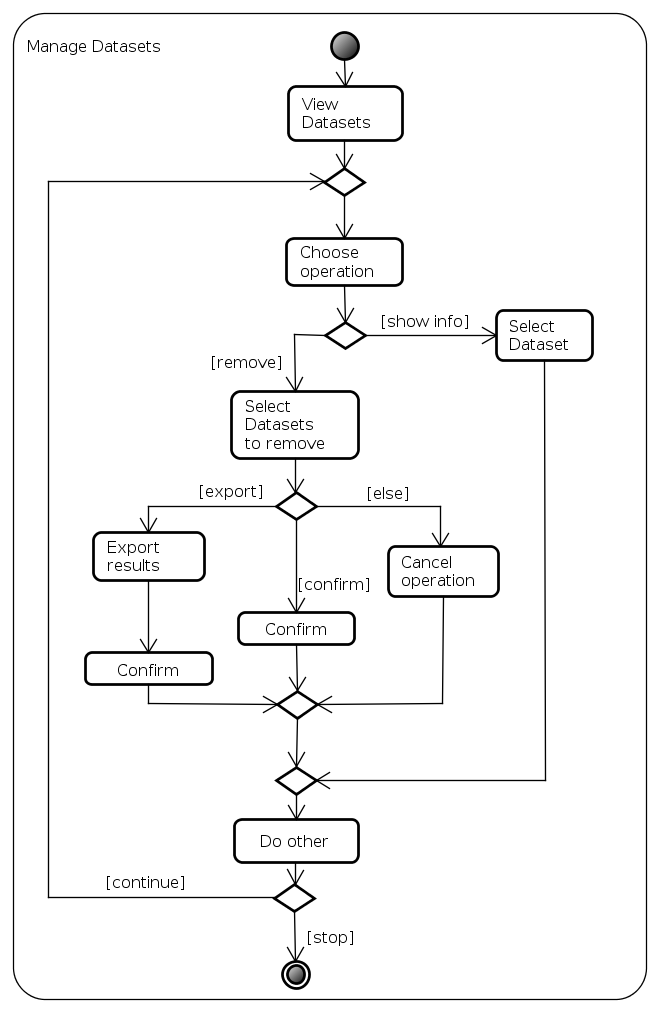
\includegraphics[width=0.85\linewidth]{./Content/Immagini/Manage_Datasets}
\caption{Diagramma Attività - Gestione dei Dataset}
\label{ManageData}
\end{figure}
\paragraph{Descrizione\\}
L'attività di gestione dei Dataset\glossario{} (fig. \ref{ManageData}), dà la possibilità all'utente di visualizzare i Dataset\glossario{} presenti in quel momento nel sistema. Per ogni \dataset{}, è possibile decidere se visualizzarne le informazioni d'interesse o se rimuoverlo. La cancellazione di un \dataset{} necessita della conferma da parte dell'utente.
\pagebreak

%avviare un'analisi
\subsection{Do an Analys}
\label{doAnalysis}
\begin{figure}[!h]
\centering
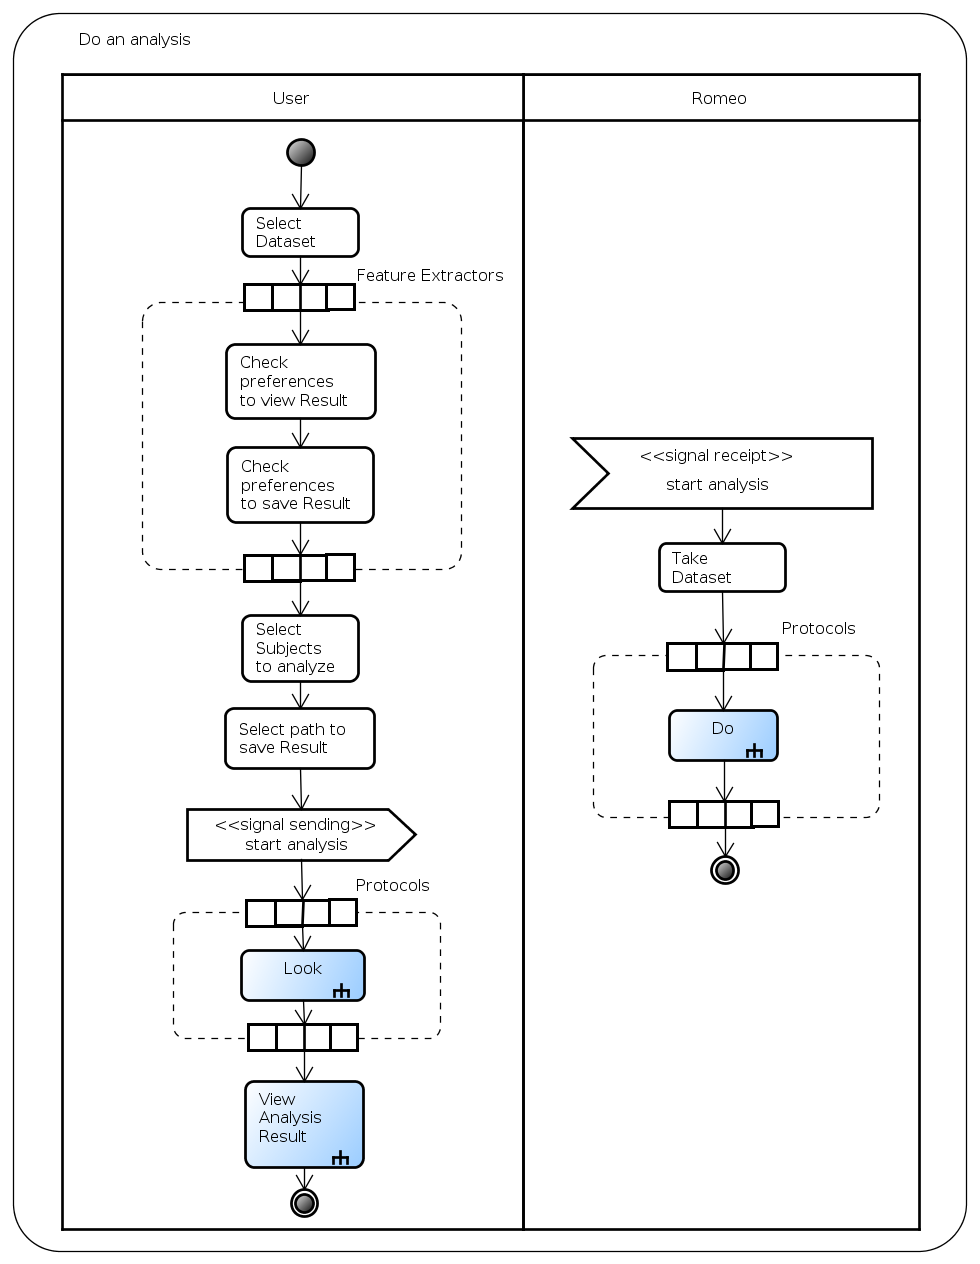
\includegraphics[width=\linewidth]{./Content/Immagini/Do_an_Analysis}
\caption{Diagramma Attività - Avvio di un'analisi}
\label{analysis}
\end{figure}
\pagebreak

%immagine del lavoro sulle feature
\begin{figure}[!h]
\centering
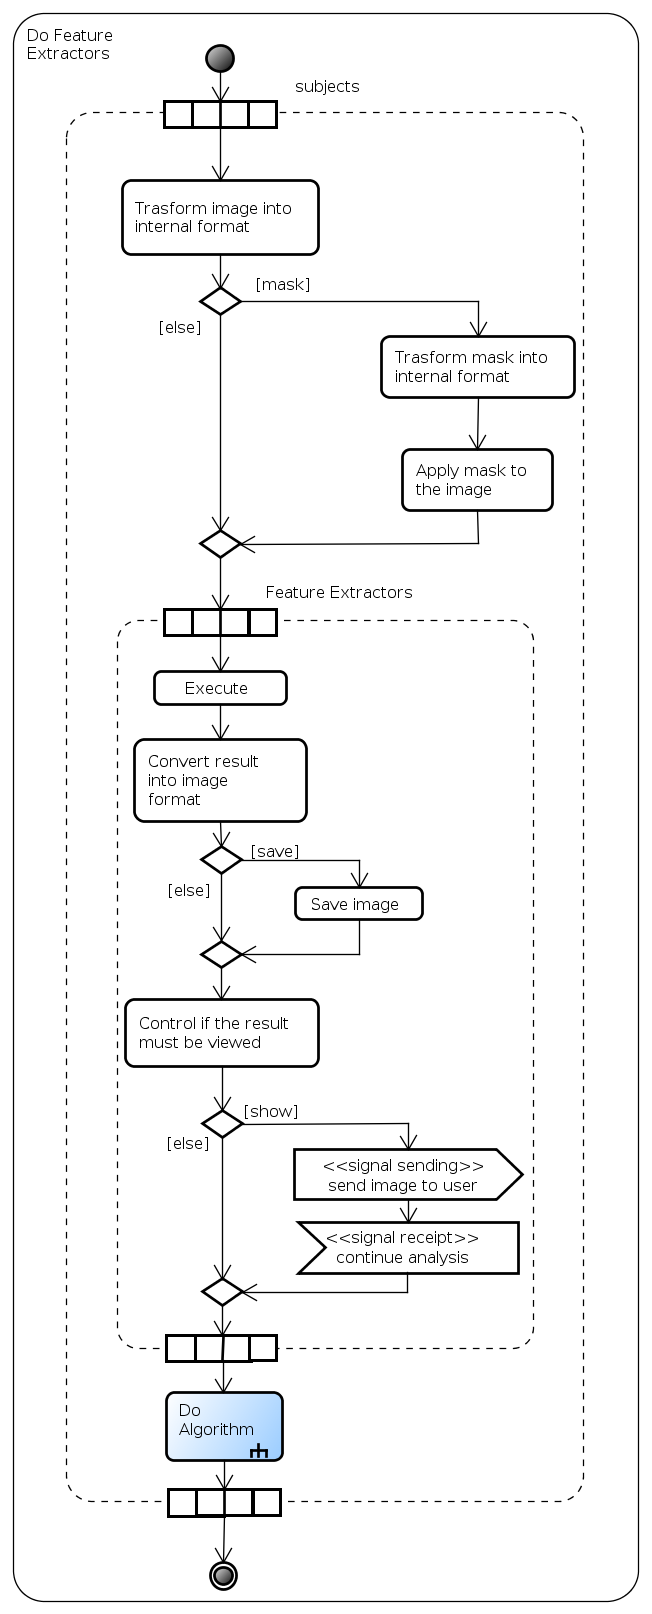
\includegraphics[width=0.65\linewidth]{./Content/Immagini/Do}
\caption{Diagramma Attività - Esecuzione analisi per ogni Protocol}
\label{DoA}
\end{figure}
\pagebreak

%immagine del lavoro dell'algoritmo
\begin{figure}[!h]
\centering
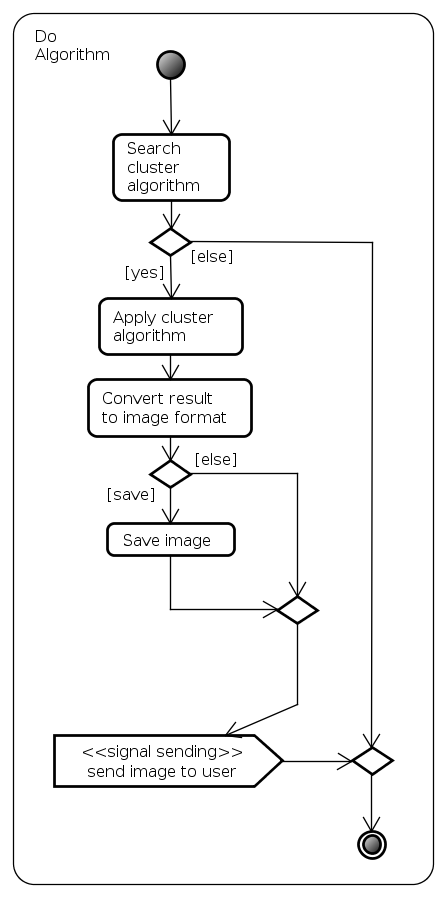
\includegraphics[width=0.48\linewidth]{./Content/Immagini/DoAl}
\caption{Diagramma Attività - Esecuzione analisi per ogni Protocol}
\label{DoB}
\end{figure}
\paragraph{Descrizione\\}
L'attività di esecuzione di un'analisi (fig. \ref{analysis}), è il processo principale del software \project{}. Per questo motivo si è scelto di rappresentare, non solo i passi che l'utente potrà fare, ma anche l'interazione vera e propria con il sistema.\\
Innanzitutto, l'utente dovrà selezionare il Dataset\glossario{} su cui vuole eseguire l'analisi. Successivamente, per ogni feature extractor\glossario{} presente nei vari Protocol\glossario{} del Dataset\glossario{}, dovrà decidere se visualizzare e se salvare il risultato dell'estrazione, subito dopo il suo calcolo. L'utente dovrà poi selezionare i Subject\glossario{} su cui vorrà effettuare l'analisi, e il path in cui vorrà salvarne i risultati.\\ Nel momento in cui l'utente fa partire l'esecuzione dell'analisi, il software eseguirà i seguenti passi per ogni \protocol{} presente nel \dataset{}:
\begin{itemize}
\item Trasforma l'immagine e l'eventuale maschera di un \subject{} nel formato interno al software;
\item Applica la maschera all'immagine (se non è presente, questo passo verrà saltato);
\item Per ogni feature extractor\glossario{} presente nel \protocol{}:
\begin{itemize}
\item Esegue l'estrazione della feature\glossario{} dell'immagine;
\item Converte il risultato dell'estrazione in immagine;
\item Salva l'immagine (questo passo viene eseguito se precedentemente scelto dall'utente);
\item Mostra l'immagine a video (questo passo viene eseguito se precedentemente scelto dall'utente)(fig. \ref{DoA});
\item Lascia decidere all'utente se continuare a visualizzare i risultati delle features extractors\glossario{} oppure continuare l'estrazione senza più mostrarli;
\end{itemize}
\item Viene eseguito l'algoritmo di clustering\glossario{} eventualmente presente nel \protocol{};
\item Il risultato verrà riconvertito in immagine;
\item L'immagine verrà salvata (condizione precedentemente decisa dall'utente);
\end{itemize}
I passi sopra elencati, verranno eseguiti per ogni \subject{} presente nel gruppo di \subject{} del \dataset{}.\\
Una volta terminata l'analisi, l'utente potrà visualizzare tutti risultati dell'analisi (vedi \ref{seeAnalysis}).
\\

%visualizzazione risultato dell'analisi
\subsubsection{Visualizzare i risultati dell'analisi}
\label{seeAnalysis}
\begin{figure}[!h]
\centering
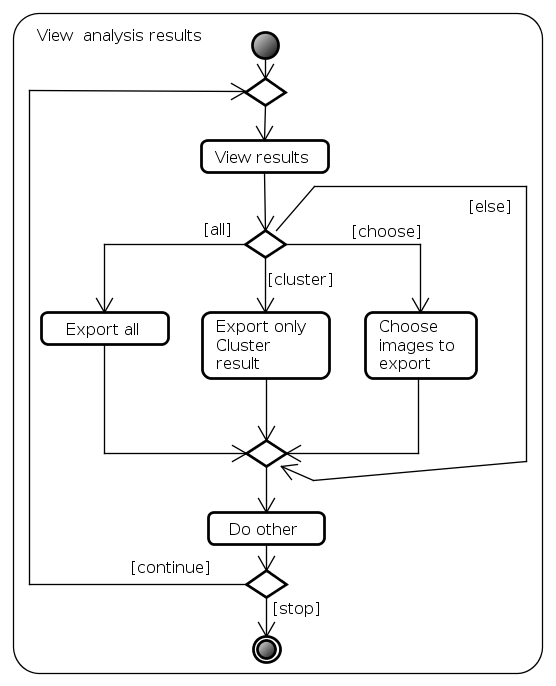
\includegraphics[width=0.6\linewidth]{./Content/Immagini/See_Analysis_Result}
\caption{Diagramma Attività - Visualizzazione dei risultati dell'analisi effettuata}
\label{showAnalysis}
\end{figure}
\paragraph{Descrizione\\}
Quest'attività, conseguente alla fine dell'analisi del \dataset{}, permette all'utente di visualizzarne i risultati. A questo punto, l'utente può decidere se esportarli o meno. Nel caso in cui li voglia esportare, può decidere se esportarli tutti, se esportare solo il risultato ultimo della cluster analysis\glossario{} oppure decidere manualmente quali immagini esportare.
\pagebreak

%visualizzazione dello storico delle analisi
\subsection{Visualizzare le analisi effettuate}
\label{ShowAll}
\begin{figure}[!h]
\centering
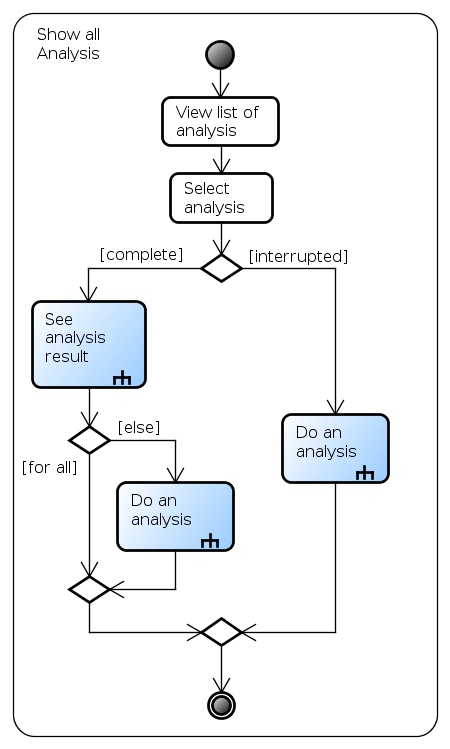
\includegraphics[width=0.6\linewidth]{./Content/Immagini/Show_All}
\caption{Diagramma Attività - Visualizzazione di tutte le analisi effettuate}
\label{showA}
\end{figure}
\paragraph{Descrizione\\}
Quest'attività permette all'utente di visualizzare lo storico delle analisi effettuate sui \dataset{} presenti nel software. Si possono presentare tre casi:
\begin{itemize}
\item L'analisi è stata completata su tutti gli elementi del gruppo di \subject{}. Sarà quindi possibile visualizzarne i risultati;
\item L'analisi è stata completata solo per un sottoinsieme di \subject{} del gruppo. In questo caso, sarà possibile visualizzarne i risultati ed eventualmente decidere di completare l'analisi sul resto degli elementi;
\item L'analisi è stata interrotta. In questo caso si ha solo la possibilità di rieseguire l'analisi (fig. \ref{analysis}).
\end{itemize}
\pagebreak

%apertura della guida
\subsection{Aprire la guida}
\label{guide}
\begin{figure}[!h]
\centering
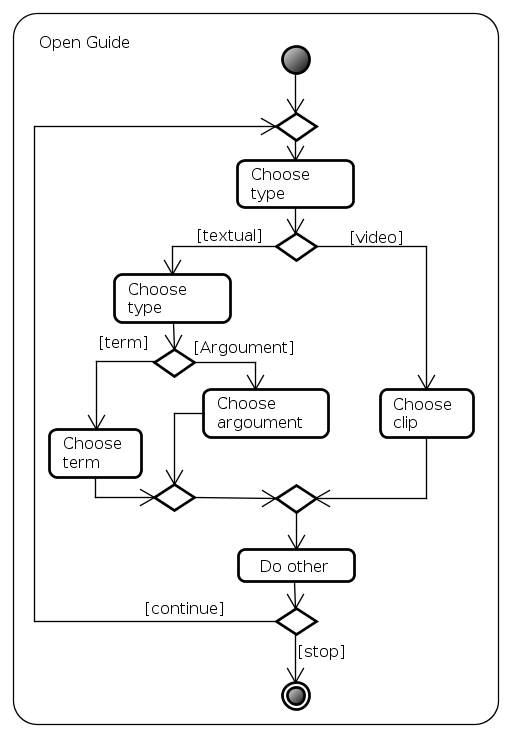
\includegraphics[width=0.6\linewidth]{./Content/Immagini/Open_Guide}
\caption{Diagramma Attività - Apertura della guida}
\label{openG}
\end{figure}
\paragraph{Descrizione\\}
L'attività di apertura della guida (fig. \ref{guide}), fornisce all'utente la possibilità di essere guidato nell'utilizzo del software \project{}. L'utente può scegliere se aprire la guida testuale oppure la guida video. Per quanto riguarda la guida testuale, ha a disposizione la ricerca per argomento oppure per termine, mentre per quanto riguarda la guida video, potrà scegliere il clip di interesse. Una volta terminata la ricerca, può continuare con una nuova ricerca oppure chiuderla.